\documentclass[10pt,twocolumn,letterpaper]{article}

\usepackage{cvpr}
\usepackage{times}
\usepackage{epsfig}
\usepackage{graphicx}
\usepackage{amsmath}
\usepackage{amssymb}

% Include other packages here, before hyperref.

% If you comment hyperref and then uncomment it, you should delete
% egpaper.aux before re-running latex.  (Or just hit 'q' on the first latex
% run, let it finish, and you should be clear).
\usepackage[breaklinks=true,bookmarks=false]{hyperref}

\cvprfinalcopy % *** Uncomment this line for the final submission

\def\cvprPaperID{****} % *** Enter the CVPR Paper ID here
\def\httilde{\mbox{\tt\raisebox{-.5ex}{\symbol{126}}}}

% Pages are numbered in submission mode, and unnumbered in camera-ready
%\ifcvprfinal\pagestyle{empty}\fi
\setcounter{page}{1}
\begin{document}

%%%%%%%%% TITLE
\title{Improved 3D U-Net for Brain Tumor Segmentation on BraTS Dataset}
\author{Dugo Alberto\\
{\tt\scriptsize alberto.dugo@studenti.unipd.it}\\
% For a paper whose authors are all at the same institution,
% omit the following lines up until the closing ``}''.
% Additional authors and addresses can be added with ``\and'',
% just like the second author.
% To save space, use either the email address or home page, not both
\and
Cecchin Andrea\\
{\tt\scriptsize andrea.cecchin.5@studenti.unipd.it}\\
\and
Soldà Matteo\\
{\tt\scriptsize matteo.solda.1@studenti.unipd.it}\\
}
\maketitle
%\thispagestyle{empty}

%%%%%%%%% ABSTRACT
\begin{abstract}
    This paper presents a deep learning framework based on the U-Net architecture for the task of brain tumor segmentation. Utilizing the publicly available BraTS Challenge dataset for training and evaluation, the proposed model leverages multimodal MRI data to generate precise segmentations of tumor regions. By addressing this critical challenge in clinical oncology within a single architecture, the approach demonstrates the potential of integrated deep learning solutions for comprehensive and clinically relevant analysis of brain tumors.
\end{abstract}

%%%%%%%%% BODY TEXT
\section{Introduction}
CBTRUS\cite{CBTRUSTumors2022} maintains and regularly updates a registry of malignant and non-malignant brain tumors.
In global data, the incidence of malignant brain tumors is approximately 3.5 per 100,000 people. This incidence increases to 3.9 for the male population and 3.1 for the female population. This indicates that approximately 173,699 men and 148,032 women are diagnosed with brain tumors each year, for a total of 321,731 individuals. The average annual mortality in the United States alone between 2017 and 2021 was 4.41 per 100,000 people. This represents a death of 17,411 people per year, or 48 deaths per day.


Brain Tumor Segmentation Challenge is an annual competition, firstly launched by the Perelman School of Medicine\cite{BraTSChallenge} in 2012, focused on evaluating the performance of algorithms in tasks related to the segmentation of brain tumors in multimodal MRI scans. In particular, our work focused on the segmentation of gliomas, which is the task of recognizing a tumor region if present.

It requires the segmentation of the three typical regions which characterize a brain tumor:
    \begin{itemize}
        \item Enhancing Tumor: it is the region of a brain tumor characterized by the presence of a disrupted blood-brain barrier.
        \item Peritumoral Edema: it is the swelling of tissue surrounding a brain tumor, caused by the accumulation of fluid.
        \item Necrotic and Non-Enhancing Tumor Core: it is the central region of a brain tumor that contains dead tissue.
\end{itemize}

Being able to correctly identify and classify tumor areas is a highly important task, because it increase the survival rate of patients. Despite that, those tasks are extremely challenging. The difficulty, and the reason why tumor segmentations are performed by human experts, lies in the challenge of visualizing certain tumor areas in MRI scans.

Indeed, while peritumoral edema is easily visible even without image preprocessing or contrast modification, the Enhancing Tumor is only visible in post-contrast scans, where it appears brighter. Even more difficult is the segmentation of the Necrotic and Non-Enhancing Tumor Core, which does not show contrast enhancement in MRI scans.

Modeling and training a deep neural network to perform these tasks would decrease the time required to accurately identify tumor regions in MRI scans, potentially increasing the accuracy of human-made segmentations.

%------------------------------------------------------------------------
\section{Related Works}

Over the past decade, deep learning has become the dominant paradigm for brain‐tumor segmentation. Early 2D CNNs such as the cascaded “Two‐Phase” network of Havaei et al.~\cite{HAVAEI201718} achieved an overall Dice of 0.86 for whole‐tumor and tumor‐core regions and 0.77 for enhancing tumor, thanks to its dual‐stream design that fuses local and global context and a two‐stage training scheme. Gordillo et al.~\cite{GORDILLO20131426} provide a comprehensive benchmarking of these early models, highlighting that most fell short on delineating the enhancing core in heterogeneous cases.

With the advent of volumetric architectures, 3D U‐Net variants quickly became the de facto standard. The original 3D U‐Net by Çiçek et al.~\cite{cicek20163dunetlearningdense} and its nnU‐Net successor by Isensee et al.~\cite{isensee2020nnunetbraintumorsegmentation} demonstrated superior generalization by self‐configuring preprocessing and training pipelines, routinely scoring $>$0.85 Dice on BraTS~\cite{dong2017automatic,bukhari2021e1d3,myronenko2019robust}. More recent lightweight adaptations, such as LIU‐Net (2021), which reduces parameters via depthwise separable convolutions, and BTIS‐Net (2022), which employs bottleneck blocks and channel pruning—achieve comparable Dice (0.84–0.86) with 60–80\% fewer parameters~\cite{Liu2024BTIS,Ahmad2025liu}. Meanwhile, hybrid and transformer‐based models such as Swin‐UNet~\cite{cao2021swinunetunetlikepuretransformer} have begun to close the gap further, offering richer global context modeling at the cost of higher computational overhead. However, there remains a need for architectures that strike an optimal balance between parameter efficiency, inference speed, and segmentation accuracy, especially for resource‐constrained clinical settings.

%-------------------------------------------------------------------------

\section{Dataset}
For this project, we used the official dataset\cite{BraTSdataset} provided for the BraTS Challenge held in 2020, obtained from the Kaggle dataset repository. The data comprises the combination of 19 different clinical datasets created using various protocols and scanners, encompassing MRI scans from 494 patients.

For each patient, four different three-dimensional brain scans are provided. T1-weighted MRI emphasizes anatomical details, providing good contrast between gray matter and white matter structures. T1 contrast-enhancing (T1ce) is acquired after gadolinium-based contrast agent administration, where the contrast accumulates in areas with high vascular permeability, causing tumors to appear brighter than surrounding tissues. The T2 scan highlights water-rich areas such as edema, while T2-FLAIR (Fluid Attenuated Inversion Recovery) suppresses cerebrospinal fluid signals, enabling better visualization of brain lesions.

\begin{figure}[H]
\centering
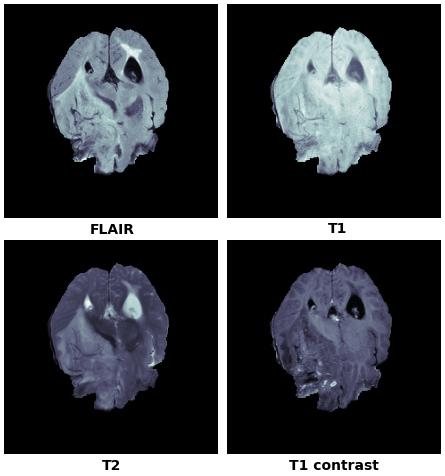
\includegraphics[width=0.55\linewidth]{img/example_MRI.png}
\caption{Example of an MRI scan with FLAIR, T1, T2 and T1 contrast-enhancing.}
\end{figure}

The images were preprocessed with all scans realigned and resampled to a uniform voxel size of 1 mm³, and non-brain tissues including skull and scalp were removed. For the 369 patients in the training set, manual segmentations of tumor areas were created, verified, and validated by expert neuroradiologists, serving as ground truth for model training and validation.

\begin{figure}[H]
\centering
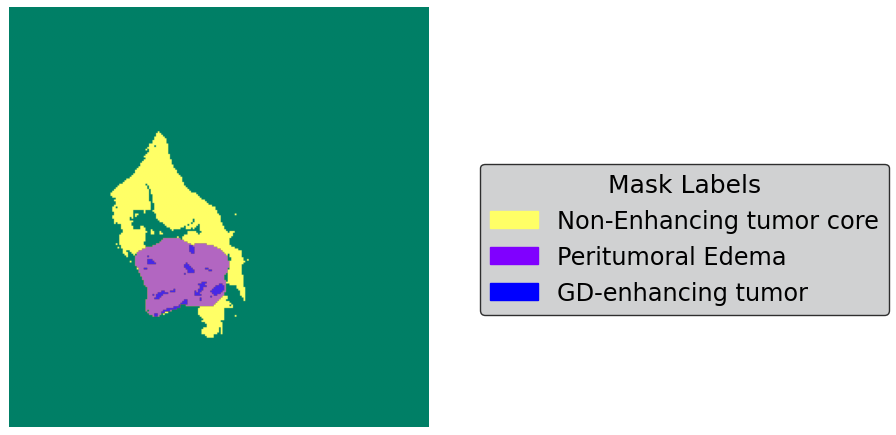
\includegraphics[width=0.65\linewidth]{img/groundtruth_example.png}
\caption{A colored version of the manual segmentation provided for a patient in the training set.}
\end{figure}

The dataset was structured for volumetric analysis with input tensors of dimensions $[B, C, H, W, D] = [2, 4, 240, 240, 155]$, where $B$ represents the batch size, $C$ corresponds to the four MRI modalities, and $H \times W \times D$ defines the spatial dimensions. Prior to model input, intensity normalization was applied independently for each modality using z-score standardization, ensuring zero mean and unit variance within the brain region.
\section{Method}
Our model implements a customized 3D U-Net architecture specifically designed for volumetric brain tumor segmentation in multimodal MRI scans.

\subsection{Architecture} \label{Architecture}
We developed an improved 3D U-Net variant with an exceptionally lightweight structure, optimized for efficient tumor subregion delineation. The network is designed to be as compact as possible while preserving high segmentation accuracy. It comprises a total of 340,596 parameters, corresponding to approximately 1.30 MB of memory during inference (assuming 32-bit floating-point precision).

The architecture follows an encoder-decoder structure with three resolution levels, 
connected via skip connections to retain spatial context. Each encoder block applies a 3D convolution (Conv3d) to process volumetric MRI data across spatial and depth dimensions, 
followed by Instance Normalization and LeakyReLU activation. 
The network is tailored for the BraTS 2020 dataset, where each input volume, as we mention before, contains four MRI modalities (T1, T1ce, T2, FLAIR), stacked as input channels. 
The initial Conv3d layer takes this 4-channel input and produces multiple feature maps, capturing localized 3D features relevant to tumor segmentation. 
Downsampling between levels is performed using 3D max pooling with a stride of 2. The decoder path mirrors the encoder, progressively upsampling and refining features to reconstruct segmentation outputs.
To mitigate overfitting, a dropout layer with a rate of $0.3$ is inserted prior to the final $1\times1\times1$ convolutional layer, which maps feature representations to the output segmentation classes. 
Model weights are initialized using Kaiming initialization, which is well-suited for networks employing LeakyReLU activations. 
Kaiming initialization \cite{He_2015_ICCV} sets the weights of each layer based on the number of input units, specifically drawing from a distribution with variance scaled by $\frac{2}{(1 + a^2)n}$, where $a$ is the negative slope of the LeakyReLU and $n$ is the number of input connections.  
This architecture demonstrates an excellent trade-off between computational efficiency and segmentation performance. With approximately 340,000 trainable parameters, the network remains lightweight and computationally tractable, making it particularly suitable for deployment in resource-constrained clinical settings. Despite its compact size, the model achieves a Dice score of 79\% on the BraTS 2020 dataset, a remarkable result that underscores the effectiveness of the design in capturing critical volumetric features for brain tumor segmentation.



\begin{figure}
    \centering
    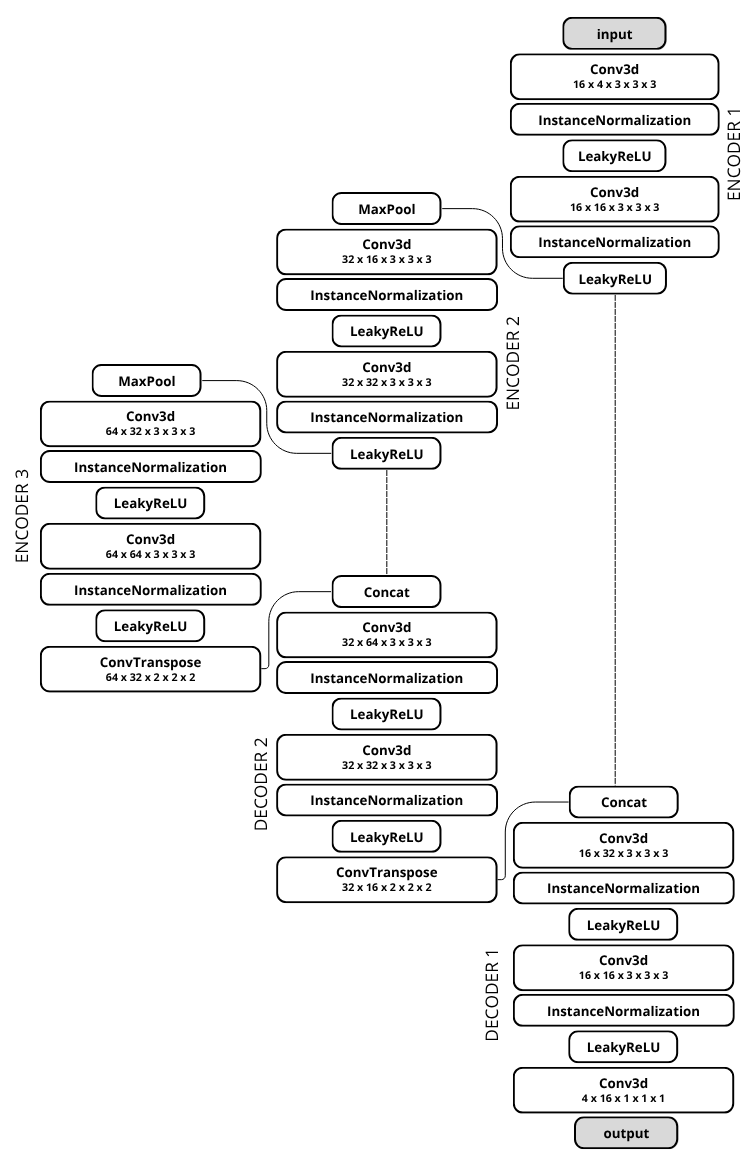
\includegraphics[width=0.8\linewidth]{img/architect.png}
    \caption{A simplified illustration of the developed architecture.}
\end{figure}


\subsection{Loss Function} \label{loss_function}
The entire training phase of our 3D U-Net is based on the use of a combined loss function. Specifically, we employed a loss function that integrates both the Cross-Entropy Loss, contributing 30\% to the final loss value, and a Dice Loss weighted at 70\%.

The Dice Loss used in our implementation is a differentiable (soft) variant of the Dice Similarity Coefficient, or Dice Score. Instead of relying on hard class assignments, it operates on class probabilities obtained after applying a softmax function to the model’s output logits. It is computed independently for each class across the entire batch, and then averaged.

\begin{equation}
\mathcal{L}_{\text{Dice}} = 1 - \frac{1}{C} \sum_{c=1}^{C} \frac{2 \sum_i p_{c,i} \cdot g_{c,i} + \epsilon}{\sum_i p_{c,i} + \sum_i g_{c,i} + \epsilon}
\end{equation}
\textit{where}\\
$C$\textit{: number of classes;}\\
$p_{c,i}$\textit{: predicted probability for class c in pixel i;}\\
$g_{c,i}$\textit{: ground truth probability for class c in pixel i;}\\
$\epsilon$\textit{: smoothing.}\\

This soft Dice Loss enables a direct and global measure of overlap between the predicted segmentation maps and the corresponding ground truth masks, reflecting how well the predicted regions match the anatomical structures of interest in the MRI scans.

In addition to optimizing spatial agreement, incorporating the Dice Loss into the training objective provides several important benefits. First, it helps mitigate the problem of class imbalance, which is common in medical image segmentation tasks where the target structures, such as tumoral area, often occupy only a small fraction of the image volume. Unlike Cross-Entropy, which gives equal weight to all pixels regardless of class frequency, Dice Loss inherently emphasizes the accurate prediction of underrepresented structures, promoting better performance on small or sparse regions.

By combining both losses, we leverage the strengths of each: the fine-grained discrimination of Cross-Entropy and the region-level accuracy of Dice, ultimately improving the overall performance of the model.

\begin{equation}
\mathcal{L}_{\text{Combined}} = 0.3 \cdot \mathcal{L}_{\text{CE}} + 0.7 \cdot \mathcal{L}_{\text{Dice}}
\end{equation}


\section{Experiments}

\subsection{Architectural Choices} \label{architectural_choices}

The model architecture selected, as described in section \ref{Architecture}, is the result of extensive experimentation involving several architectures of varying complexity and design. Each model was compared based on its performance in terms of Dice Score. This model and its weights are stored on Hugging Face and can be downloaded from the following link: \url{https://huggingface.co/dugoalberto/3D_U_Net}.
In particular, two additional, more complex architectures were developed, trained, and evaluated on the same dataset.

The first alternative architecture was a variant of the final selected one, featuring an additional fourth resolution level in the encoder path and a symmetric decoder. This version retained the same design principles, including skip connections and a residual-like structure for each block. The resulting two models, based on this, comprise a total of 2,867,956 parameters for the smallest version, and 11,465,188 in the other. Also this model is available on Hugging Face at the following link: \url{https://huggingface.co/andreacecchin/Medium_3D_U_Net}.

The second and last alternative architecture that was developed and tested includes another additional block in the encoder path, resulting in a model with five resolution levels in the encoder and four in the decoder. This architecture was used to generate two models: one that contains a total of 11,536,756 parameters, approximately 34 times more than the selected model, and the other 46,137,060, 135 times the chosen one. This last architecture is also available on Hugging Face at the following link: \url{https://huggingface.co/andreacecchin/Deep_3D_U_Net}.

The decision to test models with varying numbers of parameters was made in an effort to investigate the correlation between model performance, in terms of the Dice Score of the predicted segmentations compared to the ground truth masks, and model complexity, with the aim of identifying the optimal trade-off.

The model evaluation phase was carried out by splitting the training dataset into a training set and a validation set, using the former to train the models and the latter to assess performance in terms of Dice Score and loss function. In particular, in order to accelerate this phase, all the models were trained using a subset of slices for each MRI scans, comparing the resulted scores after 90 epochs.

Interestingly, despite the increased depth and number of parameters, the tested architectures did not yield any performance improvements over the lighter alternative, with Dice Similarity Coefficient scores remaining highly comparable across deeper models.
For this reason, the architecture with 340,596 parameters was preferred, as it offered the best trade-off between performance and computational complexity. In parallel with these experiments, different combinations of weights for Cross-Entropy and Dice Loss were attempted, leading to the final combined loss already presented in section \ref{loss_function}.

\subsection{Training}
The training process was designed to ensure stability, performance, and efficiency throughout all epochs. The model was trained using a supervised learning setup on all slices comprising the 3D MRI scans of our dataset, with paired input MRI slices and their corresponding segmentation masks as ground truth. The training loop incorporated several best practices to optimize learning and prevent overfitting or gradient-related issues, such as early stopping to avoid overfitting and gradient clipping to mitigate the risk of exploding gradients. To improve generalization, data augmentation techniques were applied through albumination, including random rotation and vertical and horizontal flipping, both with a probability of 0.5, which helped the model learn to be invariant to these transformations. This augmentation was applied to both the input MRI slices and their corresponding segmentation masks, ensuring that the model learned robust features.

After every forward pass, predictions is extracted from the model outputs and compared with the ground truth segmentation, computing loss and Dice Score to evaluate segmentation performance for each batch. The average Dice Score and training loss is computed over the entire epoch to monitor learning progress.

The validation phase follows the same structure, evaluating the model on a separate validation set using the same loss function and Dice metric.
To prevent overfitting, early stopping is implemented. The validation loss is monitored across epochs, and training is terminated early if the loss did not improve beyond a minimum threshold for a predefined number of consecutive epochs.

Specifically, we decided to use GradScaler from PyTorch to automatically scale the gradients during backpropagation, which helps prevent numerical instability and allows for larger learning rates. The model was trained using the AdamW optimizer with a starting learning rate of $5e-4$ and a weight decay of $5e-4$. The learning rate was adjusted step-by-step using a ReduceLROnPlateau scheduler, which reduces the learning rate by a factor of 0.5 if the validation loss does not improve for 2 consecutive epochs and fixing a lower bound of $1e-6$. This adaptive learning rate strategy helps the model converge more effectively by allowing it to take larger steps initially and then fine-tune as it approaches a minimum.

\begin{figure}[H]
    \centering
    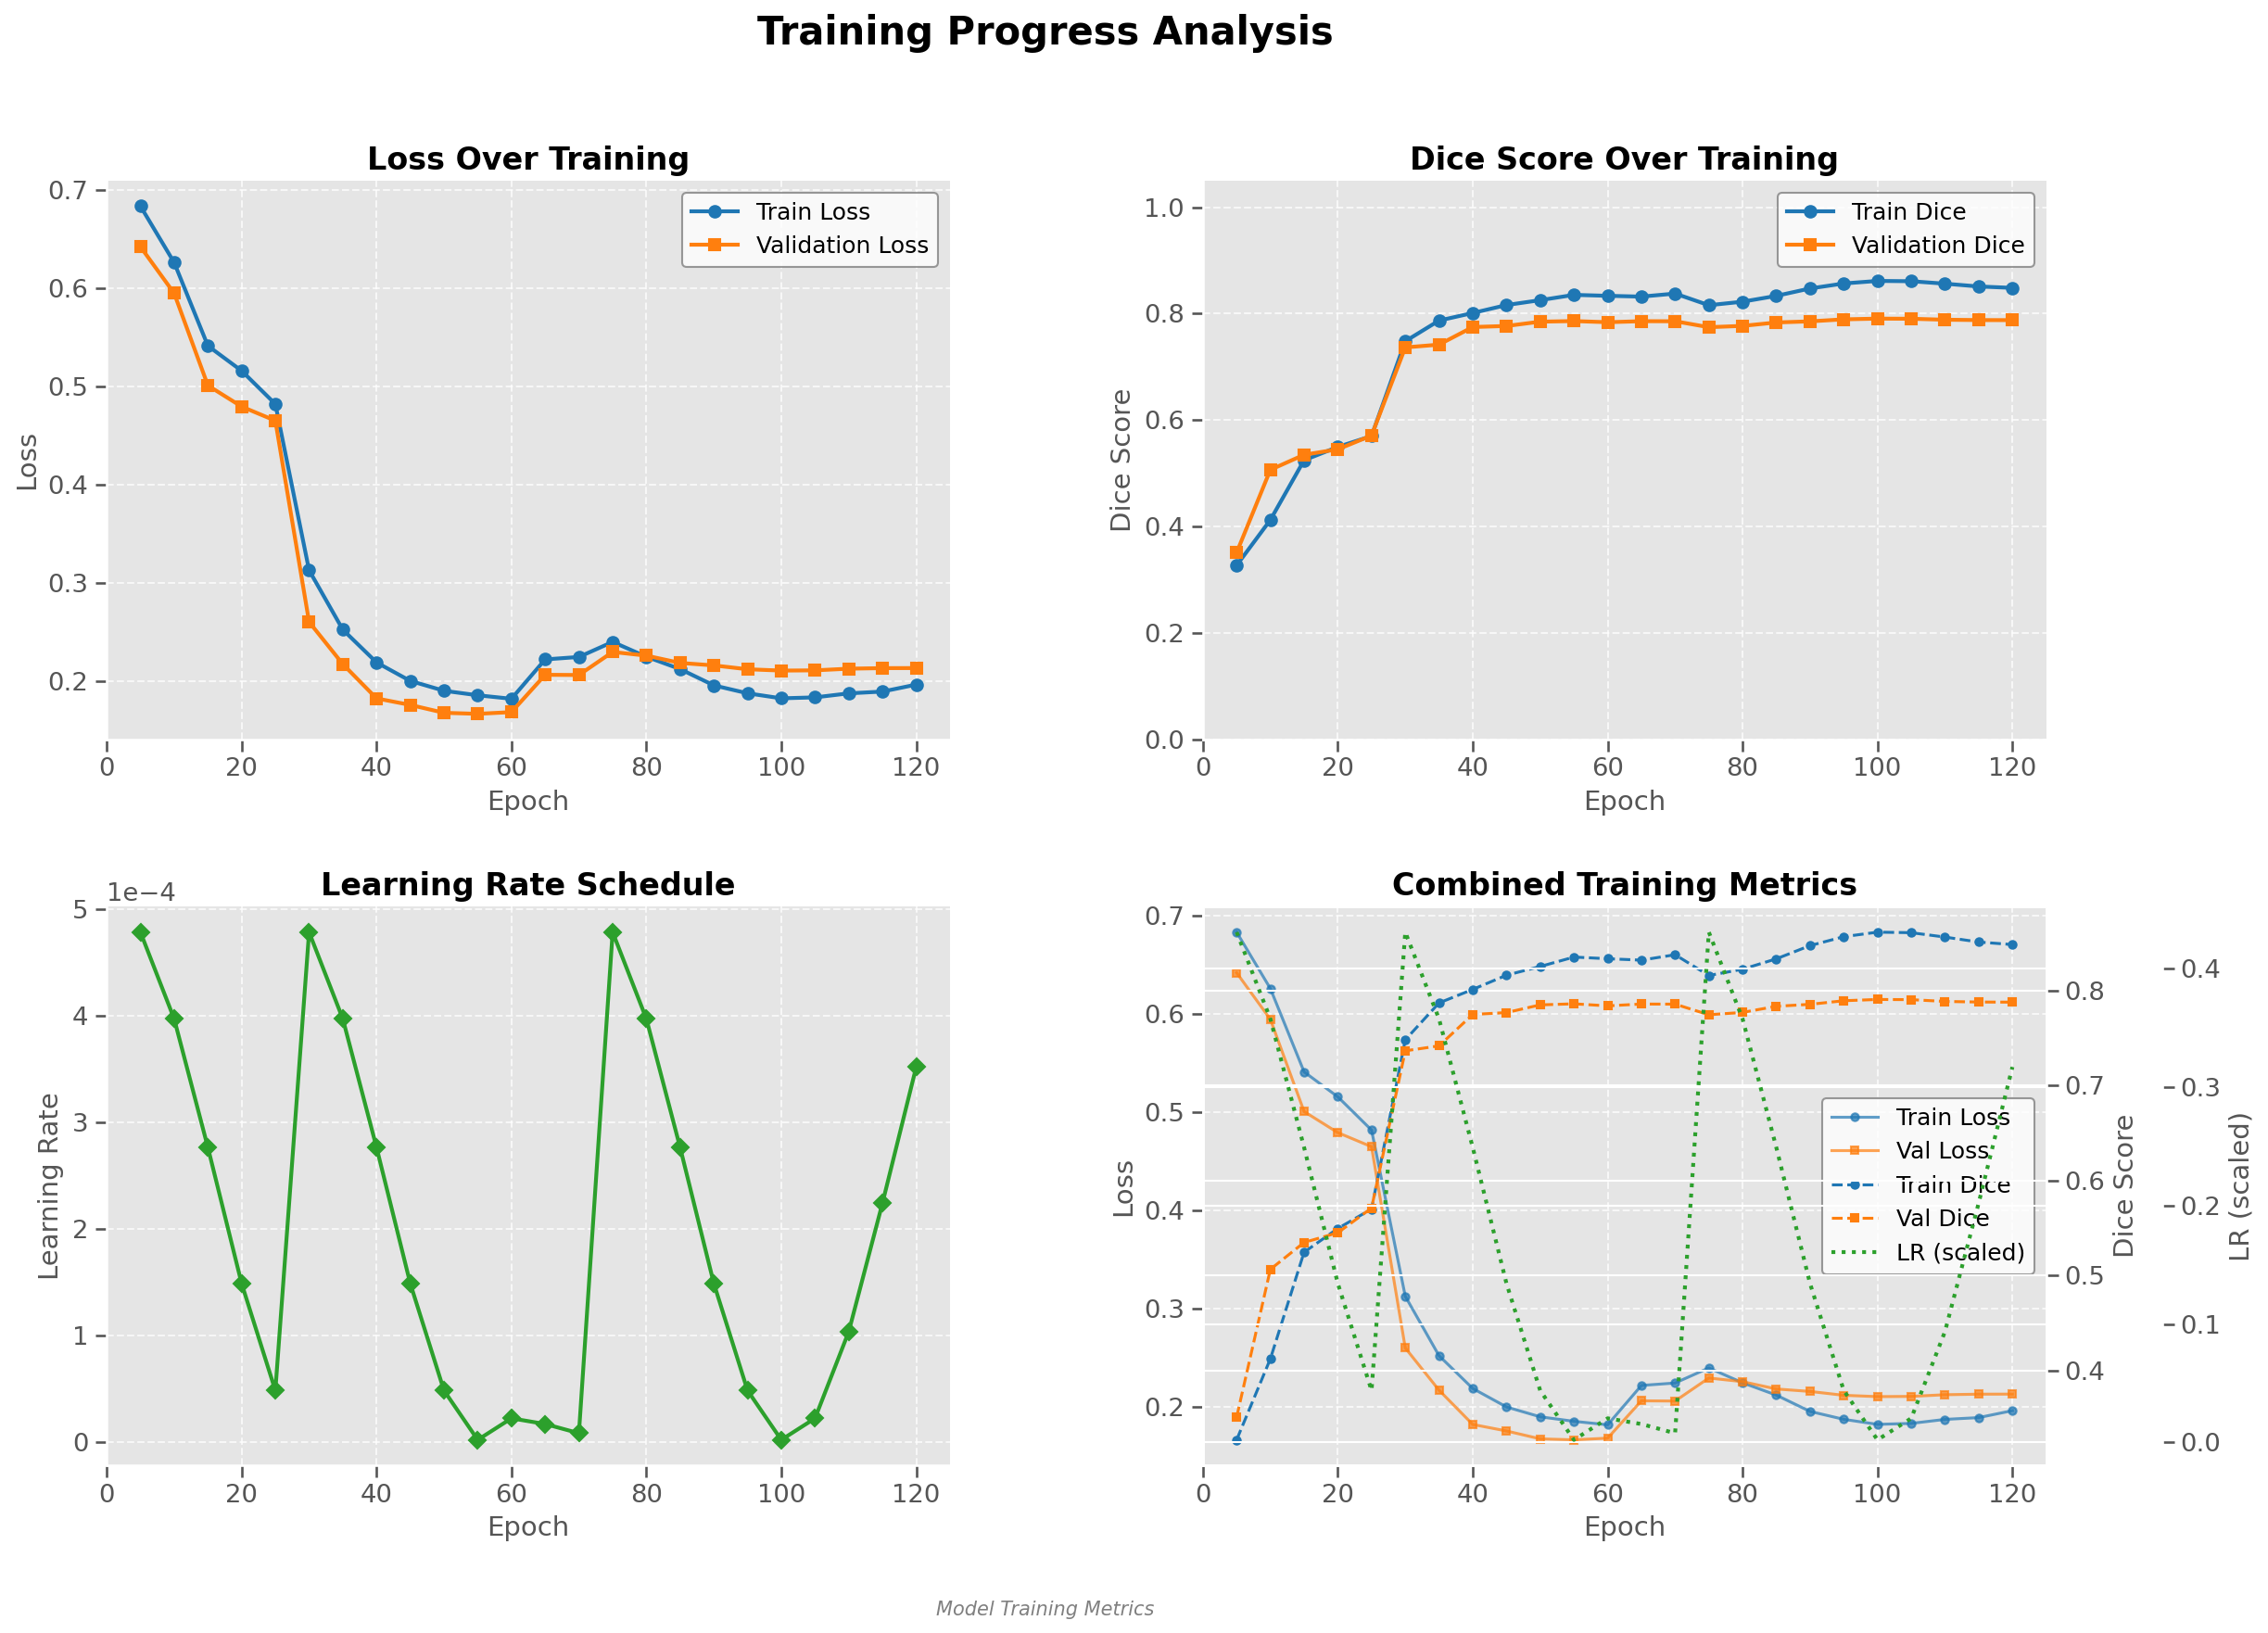
\includegraphics[width=\linewidth]{img/training4mb.png}
    \caption{Progression of Loss, Dice Score and learning rate over training epochs.}
\end{figure}

During training, model checkpoints are periodically saved every 5 epochs to allow for recovery and future analysis. In addition, a separate checkpoint is saved whenever the model achieved a new highest Dice Score on the validation set. This best-performing model, based on validation performance, is retained and ultimately selected for evaluation on the test set, ensuring that only the most effective model in terms of segmentation quality is actually used for the final inference.


\subsection{Results}
The proposed encoder-decoder architecture demonstrated substantial effeciveness in automated brain tumor segmentation using 3D MRI imaging data. The model achieved a Dice Score of 0.79 on the validation set, indicating strong overlap between predicted segmentation mask and ground truth annotations. This performance level represent a clinically relevant accuracy threshold in support of human radiologists in identifying and delineating tumor regions.
The three-class segmentation task presented significant challenges due to the distinct imaging characteristics and spatial relationships between the three tumor subregions.
The achieved Dice Score places the model within the competitive range of the modern state-of.the-art methods for brain tumor segmentation, that typically reports a score between 0.75 and 0.85.

The results of the presented model were evaluated epoch by epoch on the validation set (also because the test set was not available on Kaggle at the time of writing this paper) and compared with the results of the other two architectures presented in section \ref{architectural_choices}.
As previously mentioned, the final model had a Dice Score of 0.79 and some examples are shown in Figure \ref{fig:row-1-column-1} and \ref{fig:row-2-column-1}.

In particular: the Peritumoral Edema class achieved a combined loss of 0.7323 and a Dice Score of 0.7727; the Enhancing Tumor class achieved a loss of 0.7239 and a Dice Score of 0.8026; the Necrotic and Non-Enhancing Tumor Core class had the highest loss (1.8782) and a Dice Score of 0.6448; finally, the Background class reached a Dice Score of 0.9989 with a combined loss of 0.0031.

In addition to these metrics, we also calculated the Hausdorff95 distance, a boundary-based evaluation metric that measures the 95th percentile of the maximum distance between the predicted segmentation and the ground truth, thus quantifying how closely the predicted borders align with the reference labels. Lower values indicate better boundary agreement and higher segmentation precision. The results showed that the Background class achieved an excellent Hausdorff95 distance of 0.2464 mm, indicating near-perfect border overlap. The Enhancing Tumor, Peritumoral Edema, and Necrotic and Non-Enhancing Tumor Core classes exhibited higher Hausdorff95 distances of 5.0973 mm, 8.4238 mm, and 7.6740 mm respectively, reflecting the greater complexity and variability in accurately delineating tumor boundaries, still demonstrating acceptable performance.

Comparing our model directly with other two present in the literature, our performance aligns also with state-of-the-art lightweight methods like those reviewed pattern in \cite{An2024DWKD} and in \cite{Gutierrez2024Brain}, which also achieve competitive results with significantly fewer parameters reporting a Dice Score between 0.75 and 0.82.

In the notebook is also provided the possibility to evaluate separately every single class of the segmentation, which is useful to understand how the model performs on each of the three classes. The result can be seen at Figure \ref{tab:results}.

\begin{figure}
\centering
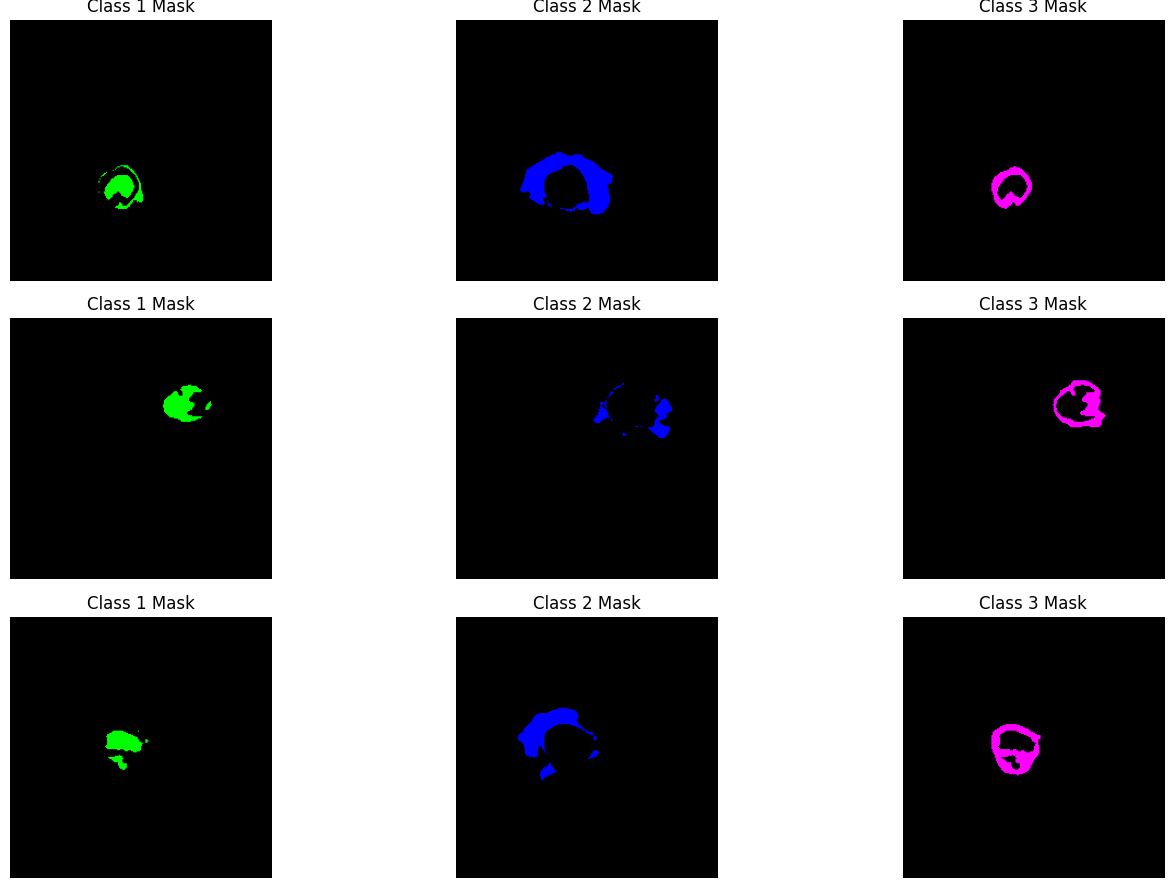
\includegraphics[width=\linewidth]{img/SeparatedColor.png}
\caption{The segmentation results of the model on the validation set, separated by class: in green the N.N.E. Core, in blue the Peritumoral Edema, in magenta the Enhancing Tumor.}
\label{tab:results}
\end{figure}


\begin{figure} 
\centering
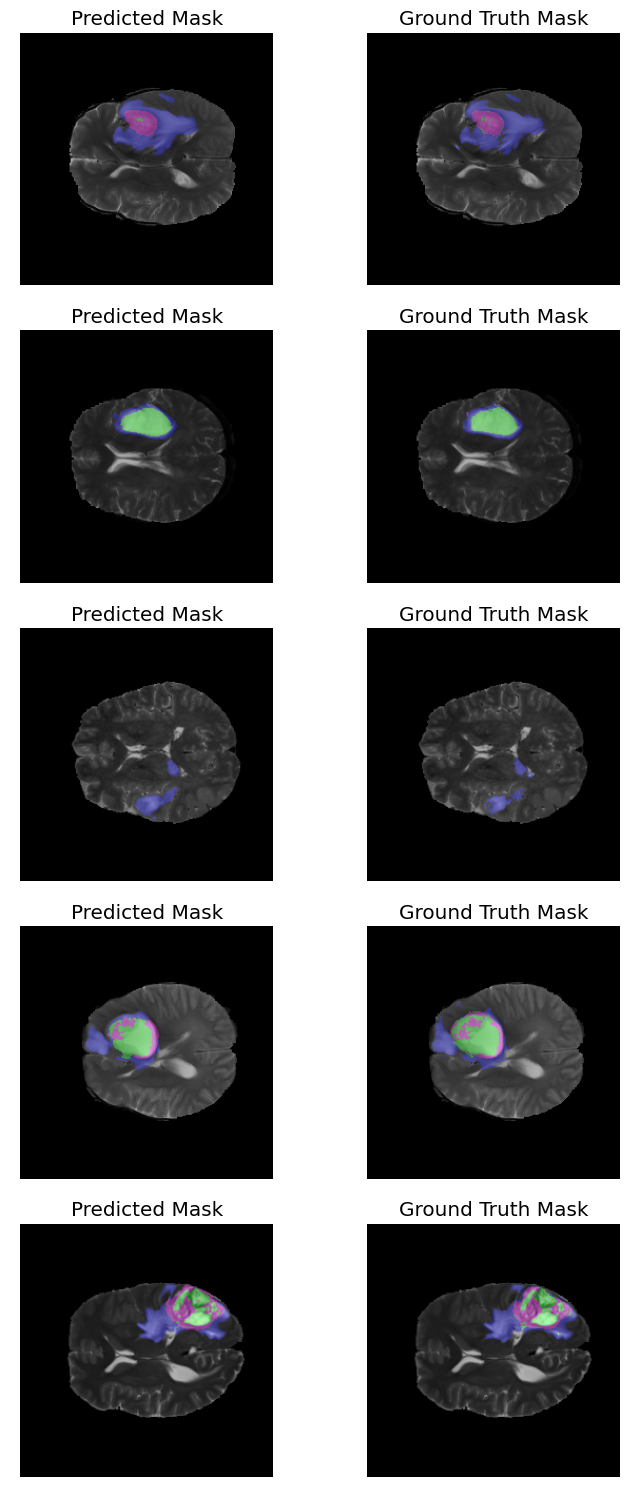
\includegraphics[width=0.8\linewidth]{img/row-1-column-1.png}
\caption{First example of segmentation results on the validation set. The first column shows the predicted segmentation, while the second column shows the ground truth segmentation.}
\label{fig:row-1-column-1}
\end{figure}

\begin{figure} 
\centering
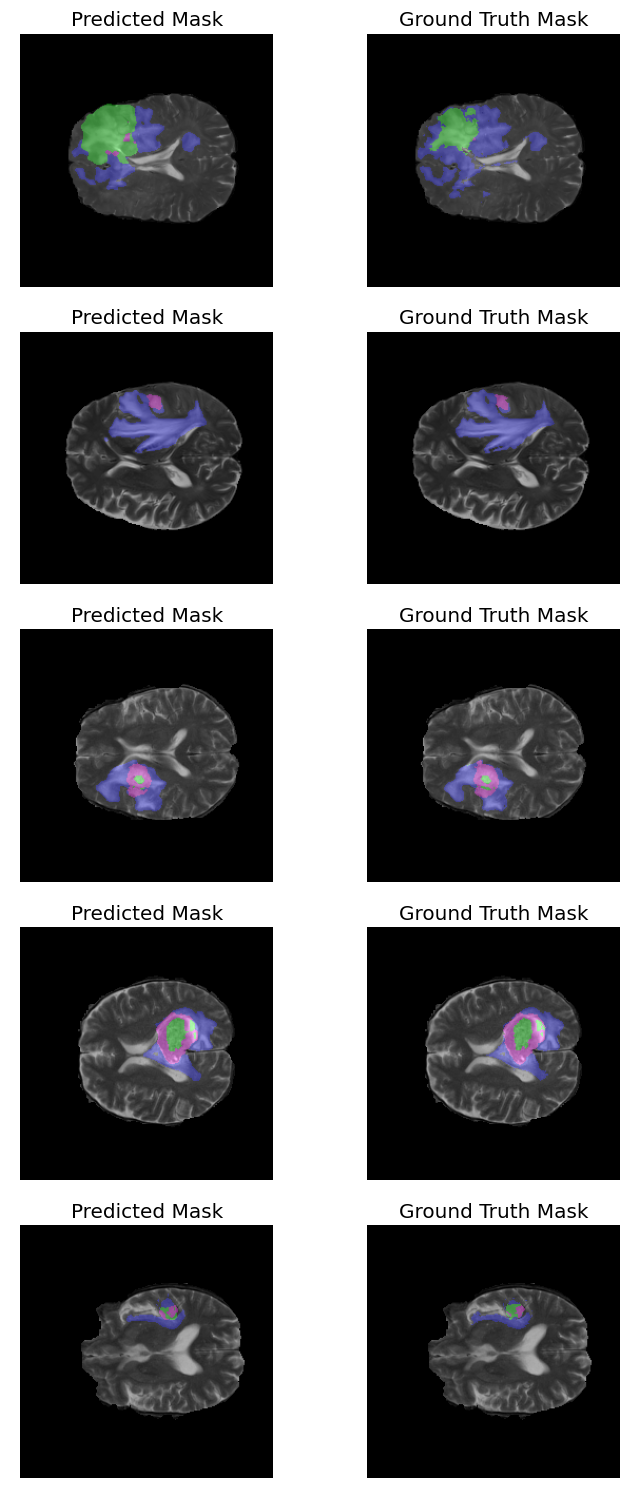
\includegraphics[width=0.8\linewidth]{img/row-2-column-1.png}
\caption{Second example of segmentation results on the validation set. The first column shows the predicted segmentation, while the second column shows the ground truth segmentation.}
\label{fig:row-2-column-1}
\end{figure}
%-------------------------------------------------------------------------
\section{Conclusions}

This works presents a lightweight 3D U-Net architecture for automated brain tumor segmentation using multimodal MRI data from the BraTS Challenge dataset. The proposed model achieved a Dice Score of 79\% with only 340.596  parameters, demonstrating that effective segmentation performance can be maintained while significalntly reducing computational complexity. The combined loss function approach, integrating Cross-Entropy and Dice Loss with weights respectively of 30\% and 70\% proved effective in addressing class imbalance challenges inherent in medical image segmentation tasks.\\\\
The clinical relevance of this research could also lead to practical deployment along the support of radiologists and oncologist in the analysis of brain tumors, potentially improving diagnostic accuracy and treatment planning also. The minimal memory footprint of 1.30MB makes the model suitable for integration into existing clinical workflow without requiring specialized hardware infrastructure.\\\\
Future work should address several key areas for improvement and extension. First of all, validation on diverse clinical datasets beyond BraTS Challenge data would establish the generalizability of the proposed architecture across different imaging protocols and patient populations.\\ Then, the second point, investigation of advanced data augmentation techniques could potentially improve model robustness and performance on edge cases.\\ And lastly, the integration of attention mechanisms within the lightweight framework could enhance the model's ability to focus on critical tumor boundary regions without significantly increasing computational overhead. \\\\
The development of ensemble methods combining multiple lightweight models could also be investigated to potentially improve overall segmentation accuracy while maintaining computational efficiency. 

%-------------------------------------------------------------------------

{\small
\bibliographystyle{ieee_fullname}
\bibliography{bibliography}
}

\end{document}
